\documentclass[a4paper,oneside,12pt]{report}
\usepackage{fontspec}
\usepackage{setspace}
\usepackage{amsmath}
\usepackage{titling}
\usepackage{geometry}
\usepackage{listings}
\usepackage{xcolor}
\usepackage{float}
\usepackage{graphicx}
\usepackage{xurl}
\usepackage{hyperref}
\usepackage{indentfirst}
\usepackage{fancyhdr}
\usepackage{tocloft}
\usepackage{bookmark}
\usepackage{booktabs}
\usepackage{caption}
\usepackage{microtype}

\emergencystretch=3em
\hfuzz=1.5pt

\setmainfont{texgyretermes-regular.otf}[
    BoldFont=texgyretermes-bold.otf,
    ItalicFont=texgyretermes-italic.otf,
    BoldItalicFont=texgyretermes-bolditalic.otf
]
\onehalfspacing
\geometry{left=3cm, right=2.5cm, top=2cm, bottom=2.5cm}
\sloppy

\definecolor{codegreen}{rgb}{0,0.6,0}
\definecolor{codegray}{rgb}{0.5,0.5,0.5}
\definecolor{codepurple}{rgb}{0.58,0,0.82}
\definecolor{backcolour}{rgb}{0.96,0.96,0.94}
\definecolor{darkblue}{rgb}{0,0,0.6}

\lstdefinestyle{commonstyle}{
    backgroundcolor=\color{backcolour},
    breakatwhitespace=false,
    breaklines=true,
    captionpos=b,
    keepspaces=true,
    numbers=left,
    numbersep=5pt,
    showspaces=false,
    showstringspaces=false,
    showtabs=false,
    tabsize=2,
    frame=single,
    basicstyle=\ttfamily\footnotesize,
    numberstyle=\tiny\color{codegray},
    columns=flexible,
    postbreak=\mbox{\textcolor{red}{$\hookrightarrow$}\space},
    breakindent=0pt,
    breakautoindent=false
}
\lstdefinestyle{bashstyle}{
    style=commonstyle,
    language=bash,
    commentstyle=\color{codegreen},
    keywordstyle=\color{darkblue},
    stringstyle=\color{codepurple}
}
\lstdefinestyle{yamlstyle}{
    style=commonstyle,
    commentstyle=\color{codegreen},
    keywordstyle=\color{darkblue},
    stringstyle=\color{codepurple}
}
\lstdefinestyle{phpstyle}{
    style=commonstyle,
    language=PHP,
    commentstyle=\color{codegreen},
    keywordstyle=\color{darkblue},
    stringstyle=\color{codepurple}
}
\lstdefinestyle{jsonstyle}{
    style=commonstyle,
    commentstyle=\color{codegreen},
    keywordstyle=\color{darkblue},
    stringstyle=\color{codepurple}
}

\newcommand{\customfbox}[1]{%
  \setlength{\fboxsep}{0pt}%
  \setlength{\fboxrule}{0.5pt}%
  \fbox{#1}%
}

\renewcommand{\figurename}{Gambar}
\renewcommand{\thefigure}{\arabic{figure}}
\renewcommand{\lstlistingname}{Listing}
\AtBeginDocument{\renewcommand{\thelstlisting}{\arabic{lstlisting}}}
\hypersetup{
    colorlinks=true,
    linkcolor=black,
    citecolor=black,
    filecolor=black,
    urlcolor=blue
}

\pagestyle{fancy}
\fancyhf{}
\fancyhead[R]{\thepage}
\renewcommand{\headrulewidth}{0pt}
\fancypagestyle{plain}{
    \fancyhf{}
    \fancyhead[R]{\thepage}
    \renewcommand{\headrulewidth}{0pt}
}

\setlength{\cftbeforetoctitleskip}{0pt}
\setlength{\cftaftertoctitleskip}{20pt}
\renewcommand{\cfttoctitlefont}{\hfill\Large\bfseries}
\renewcommand{\cftaftertoctitle}{\hfill}

\renewcommand{\cftchapleader}{\cftdotfill{\cftdotsep}}
\renewcommand{\cftsecleader}{\cftdotfill{\cftdotsep}}
\renewcommand{\cftsubsecleader}{\cftdotfill{\cftdotsep}}

\setlength{\cftchapnumwidth}{2.5em}
\setlength{\cftsecnumwidth}{2.8em}
\setlength{\cftsubsecnumwidth}{3.2em}
\renewcommand{\cftchappresnum}{}
\renewcommand{\cftchapaftersnum}{}
\newcommand{\tocboldsection}[1]{%
  \protect\renewcommand{\protect\cftchapfont}{\protect\bfseries}%
  #1%
  \protect\renewcommand{\protect\cftchapfont}{}%
}

\begin{document}

\newgeometry{left=2.5cm, right=2.5cm, top=2.5cm, bottom=2.5cm}
\begin{titlepage}
    \centering
    \vspace*{0.2cm}
    {\Large\bfseries LAPORAN PRAKTIKUM KEPL}\\[0.3cm]
    {\large\bfseries TUGAS 6: PENGALIHAN LOG STDOUT, LOG TERSTRUKTUR, ENDPOINT /HEALTH, DAN HEALTHCHECK DUA ARAH DOCKER COMPOSE}\\[2cm]

    
\includegraphics[width=0.45\textwidth]{images/UGM.png}\\[2cm]

    {\large\bfseries Disusun oleh:}\\[0.2cm]
    {\bfseries Hafidz Rizqullah Prasetya}\\[0.1cm]
    {\bfseries NIM: 24/535493/SV/24243}\\[0.1cm]
    {\bfseries Kelas: PL5A1}\\[1.5cm]

    {\large Dosen Pengampu:\\[0.2cm]
    \bfseries Galih Damaraji, S.Kom., M.Cs.}\\[1.5cm]

    \vfill
    {\bfseries PROGRAM STUDI SARJANA TERAPAN\\PENGEMBANGAN PERANGKAT LUNAK TERDISTRIBUSI\\DEPARTEMEN TEKNIK ELEKTRO DAN INFORMATIKA\\SEKOLAH VOKASI\\UNIVERSITAS GADJAH MADA\\YOGYAKARTA\\2026}
\end{titlepage}
\restoregeometry

\thispagestyle{empty}
\clearpage
\stepcounter{page}
\thispagestyle{empty}

\addcontentsline{toc}{chapter}{Daftar Isi}
\tableofcontents
\clearpage

\pagenumbering{arabic}
\setcounter{page}{3}

\chapter{Tujuan dan Lingkup Praktikum}

\section{Tujuan Praktikum}
Tujuan pelaksanaan praktikum Tugas 6 mata kuliah Konstruksi dan Evolusi Perangkat Lunak ini adalah:
\begin{enumerate}
    \item Mahasiswa mampu mengonfigurasi kanal pencatatan log pada kerangka kerja Laravel agar dialihkan langsung ke aliran standar keluaran (\texttt{stdout}) di dalam kontainer, sehingga log dapat dikelola secara terpusat oleh mesin Docker.
    \item Mahasiswa mampu merancang dan menerapkan sekurang-kurangnya tiga log terstruktur dengan konteks lengkap (pelaku, aktivitas, dan alasan terjadinya kejadian) pada alur penting aplikasi tanpa mencatat data rahasia maupun informasi pribadi.
    \item Mahasiswa mampu membangun endpoint inspeksi kesehatan sistem (\texttt{/health}) yang memverifikasi kesiapan operasional basis data relasional PostgreSQL dan subsistem penyimpanan \textit{cache}.
    \item Mahasiswa mampu mendefinisikan mekanisme \textit{healthcheck} deklaratif pada berkas \texttt{compose.yaml} dengan parameter interval, batas waktu (\textit{timeout}), jumlah percobaan ulang (\textit{retries}), dan periode pemanasan (\textit{start\_period}).
    \item Mahasiswa mampu membuktikan keandalan mekanisme pemulihan dua arah ketika layanan basis data dimatikan secara sengaja hingga kontainer berstatus \textit{unhealthy}, serta mengamati pemulihan kembali ke status \textit{healthy} setelah layanan dinyalakan ulang.
    \item Mahasiswa mampu mengonfigurasi pembatasan ukuran berkas log kontainer menggunakan opsi \texttt{max-size} dan \texttt{max-file} pada pengaturan \textit{logging} Docker Compose.
\end{enumerate}

\section{Batasan Masalah dan Repositori Kode}
Pengerjaan tugas ini melanjutkan repositori ujian tengah semester (UTS) berbasis Docker Compose yang mengelola Sistem Inventaris Aset Laboratorium TRPL. Seluruh perubahan kode aplikasi, konfigurasi lingkungan, skrip pengujian fitur, serta berkas orkestrasi kontainer dikelola pada repositori publik GitHub:
\begin{center}
    \url{https://github.com/hafidzrizqullahprasetya/uts-p1-535493}
\end{center}
Layanan aplikasi terdiri dari peladen backend berbasis FrankenPHP (PHP 8.5.12 Alpine) yang menyajikan RESTful API, basis data PostgreSQL 18.6, dan antarmuka frontend Vue.js 3 berbasis peladen Nginx.

\clearpage

\chapter{Dasar Teori}

\section{Prinsip Logging pada Arsitektur Kontainer}
Metodologi \textit{Twelve-Factor App} pada poin kesebelas menyatakan bahwa aplikasi modern tidak boleh mengelola berkas pencatatan log secara mandiri di dalam sistem berkas lokalnya. Menulis log ke berkas statis di dalam kontainer menimbulkan beberapa kelemahan kritis: log hilang saat kontainer dihancurkan, menyulitkan proses rotasi berkas, dan memicu kebocoran memori penyimpanan disk pada lingkungan produksi \cite{twelve-factor}.

Sebagai gantinya, aplikasi wajib mengalirkan seluruh pesan log kejadian ke aliran standar keluaran (\texttt{stdout}) atau standar galat (\texttt{stderr}) tanpa \textit{buffering}. Mesin kontainer seperti Docker secara otomatis menangkap aliran tersebut dan mengarahkannya ke \textit{logging driver} yang telah ditentukan, seperti \texttt{json-file}, \texttt{syslog}, atau penyedia agregasi log terpusat \cite{docker-logging}.

\section{Log Terstruktur dan Perlindungan Data Sensitif}
Pencatatan log berbasis teks bebas seringkali menyulitkan proses pemfilteran, analisis tren, dan pelacakan akar masalah saat terjadi insiden. Pendekatan log terstruktur (\textit{structured logging}) menyusun setiap entri log ke dalam format pasangan kunci dan nilai, biasanya direpresentasikan dalam JSON atau larik terindeks PSR-3 \cite{monolog}.

Setiap entri log wajib membawa metadata kontekstual yang menjawab tiga pertanyaan mendasar:
\begin{enumerate}
    \item \textbf{Siapa}: Identitas entitas yang memicu kejadian (misalnya pengenal pengguna atau agen sistem).
    \item \textbf{Aktivitas}: Operasi teknis atau alur bisnis yang sedang dijalankan.
    \item \textbf{Sebab}: Alasan terjadinya status tersebut, baik berupa keberhasilan eksekusi maupun pesan galat dari pengecualian sistem.
\end{enumerate}
Dalam implementasinya, prinsip perlindungan data pribadi dan kerahasiaan sistem wajib ditegakkan secara ketat. Berkas log dilarang keras memuat kata sandi teks biasa, token otentikasi Sanctum, kunci sesi, maupun data identitas pribadi warga negara \cite{owasp-logging}.

\section{Mekanisme Pemeriksaan Kesehatan (Healthcheck Endpoint)}
Endpoint \texttt{/health} berfungsi sebagai indikator kesiapan operasional (\textit{readiness probe}) dan ketahanan hidup (\textit{liveness probe}) dari sebuah layanan web. Endpoint kesehatan yang baik tidak boleh sekadar mengembalikan string teks statis, melainkan wajib menjalankan pemeriksaan aktif terhadap dependensi kritis yang menopang aplikasi \cite{docker-healthcheck}.

Apabila seluruh komponen inti, seperti koneksi basis data relasional dan pustaka penyimpanan \textit{cache}, dapat dihubungi dan membalas perintah uji coba dengan benar, endpoint merespons dengan kode status HTTP 200 OK. Namun jika salah satu komponen pendukung mengalami kegagalan, endpoint wajib mengembalikan kode status HTTP 503 Service Unavailable disertai laporan diagnostik yang menyebutkan secara spesifik komponen mana yang bermasalah.

\section{Orkestrasi Healthcheck Dua Arah pada Docker Compose}
Docker Compose menyediakan instrumen deklaratif untuk memantau status kesehatan kontainer secara berkala melalui blok \texttt{healthcheck}. Konfigurasi ini memiliki empat parameter utama:
\begin{enumerate}
    \item \texttt{interval}: Frekuensi eksekusi perintah pemeriksaan (misalnya setiap 10 detik).
    \item \texttt{timeout}: Batas durasi maksimal yang diberikan bagi perintah pemeriksaan sebelum dianggap gagal (misalnya 5 detik).
    \item \texttt{retries}: Ambang batas kegagalan beruntun yang diperlukan sebelum Docker mengubah status kontainer dari \textit{healthy} menjadi \textit{unhealthy}.
    \item \texttt{start\_period}: Masa tenggang awal saat kontainer pertama kali dinyalakan agar proses inisialisasi aplikasi tidak langsung divonis gagal.
\end{enumerate}
Pemeriksaan dua arah berarti status kontainer dapat berpindah secara dinamis: dari sehat menjadi sakit saat dependensi eksternal terputus, dan otomatis kembali sehat saat dependensi tersebut pulih tanpa memerlukan pembuatan ulang kontainer secara manual \cite{docker-compose-spec}.

\clearpage

\chapter[\texorpdfstring{\tocboldsection{Hasil dan Pembahasan}}{Hasil dan Pembahasan}]{Hasil dan Pembahasan}

\section{Pengalihan Kanal Log Laravel ke Stdout (Soal 1)}
Konfigurasi pencatatan log bawaan kerangka kerja Laravel secara default menggunakan kanal \texttt{stack} yang menyimpan berkas fisik ke direktori \texttt{storage/logs/laravel.log}. Untuk mengalihkan pencatatan log agar langsung keluar ke aliran standar kontainer, saluran baru bernama \texttt{stdout} ditambahkan pada berkas \texttt{backend/config/logging.php} seperti ditunjukkan pada Listing \ref{lst:config-logging}.

\begin{lstlisting}[style=phpstyle,caption={Penambahan channel stdout pada backend/config/logging.php.},label={lst:config-logging}]
'stdout' => [
    'driver' => 'monolog',
    'level' => env('LOG_LEVEL', 'debug'),
    'handler' => StreamHandler::class,
    'handler_with' => [
        'stream' => 'php://stdout',
    ],
    'formatter' => env('LOG_STDOUT_FORMATTER'),
    'processors' => [PsrLogMessageProcessor::class],
],
\end{lstlisting}

Variabel lingkungan \texttt{LOG\_CHANNEL} pada berkas konfigurasi \texttt{compose.yaml} dan berkas \texttt{.env} diatur bernilai \texttt{stdout}. Dengan demikian, setiap pesan log yang dicatat oleh aplikasi langsung ditulis ke \texttt{php://stdout} dan ditangkap oleh peladen FrankenPHP untuk kemudian dialirkan ke mesin Docker.

Bukti keluaran log yang keluar langsung ke aliran kontainer diperiksa melalui terminal dengan mengeksekusi perintah \texttt{docker compose logs backend --tail 22}. Gambar \ref{fig:log-stdout} memperlihatkan log akses HTTP dari Caddy beserta log aplikasi Laravel yang muncul secara runtut di konsol tanpa tersimpan pada disk kontainer.

\begin{figure}[htbp]
    \centering
    \customfbox{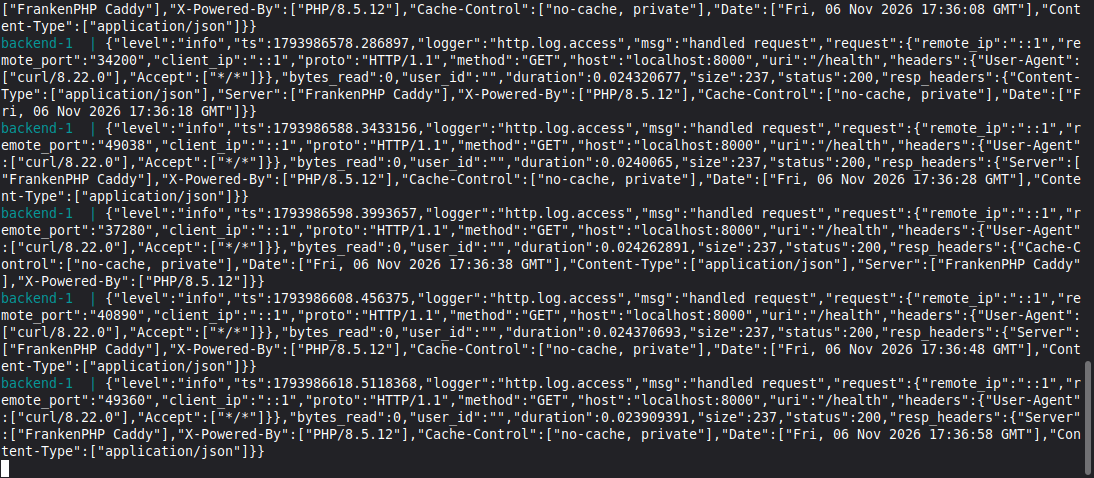
\includegraphics[width=0.98\linewidth,keepaspectratio]{images/ss-01-log-stdout-docker.png}}
    \caption{Bukti keluaran log backend tertangkap langsung melalui perintah \texttt{docker compose logs}.}
    \label{fig:log-stdout}
\end{figure}

\section{Penerapan Tiga Log Terstruktur Berkonteks (Soal 2)}
Sesuai instruksi soal, tiga alur penting pada aplikasi ditambahkan pencatatan log terstruktur menggunakan pustaka Monolog bawaan Laravel (\texttt{Illuminate\textbackslash Support\textbackslash Facades\textbackslash Log}). Setiap log memuat konteks pelaku (\texttt{siapa}), kegiatan (\texttt{sedang\_mengerjakan}), dan penjelasan kejadian (\texttt{sebab}).

\subsection{Alur 1: Penyimpanan Data Aset Baru (INFO)}
Pencatatan log tingkat \texttt{info} diletakkan pada metode \texttt{store()} di dalam \texttt{AssetController}. Log ini dipicu sesaat setelah entitas aset baru berhasil tersimpan ke dalam tabel basis data. Konteks yang dicatat mencakup email pengguna yang terotentikasi, pengenal unik aset (\texttt{id\_aset}), kode inventaris, dan kategori perangkat.

\begin{lstlisting}[style=phpstyle,caption={Potongan log info saat data aset berhasil disimpan.},label={lst:log-info}]
Log::info('Data aset berhasil disimpan', [
    'siapa' => $request->user()?->email ?? 'pengguna_terautentikasi',
    'sedang_mengerjakan' => 'menyimpan_data_aset',
    'sebab' => 'Penyimpanan data aset baru ke basis data selesai',
    'id_aset' => $asset->id,
    'kode_aset' => $asset->code,
    'kategori' => $asset->category,
]);
\end{lstlisting}

\subsection{Alur 2: Validasi Masukan Formulir Gagal (WARNING)}
Pencatatan log tingkat \texttt{warning} dipasang pada blok evaluasi validator permintaan pembuatan aset baru. Apabila atribut wajib tidak disertakan atau format tidak sesuai, sistem mencatat kejadian tersebut sebelum mengembalikan kode status HTTP 422 Unprocessable Content. Untuk menjaga keamanan data, konteks yang disimpan hanya berupa daftar nama kolom yang tidak memenuhi syarat validasi (\texttt{kolom\_gagal}), tanpa mencatat isi teks masukan pengguna.

\begin{lstlisting}[style=phpstyle,caption={Potongan log warning saat validasi masukan gagal.},label={lst:log-warning}]
if ($validator->fails()) {
    Log::warning('Validasi data aset gagal', [
        'siapa' => $request->user()?->email ?? 'pengguna',
        'sedang_mengerjakan' => 'validasi_penyimpanan_aset',
        'sebab' => 'Atribut masukan tidak memenuhi aturan validasi',
        'kolom_gagal' => array_keys($validator->errors()->toArray()),
    ]);
    return response()->json([
        'message' => 'Validasi gagal',
        'errors' => $validator->errors(),
    ], 422);
}
\end{lstlisting}

\subsection{Alur 3: Kegagalan Koneksi Basis Data (ERROR)}
Pencatatan log tingkat \texttt{error} diterapkan pada blok penanganan pengecualian (\textit{exception handling}) pada controller pemeriksaan kesehatan (\texttt{HealthController}) serta metode manipulasi aset. Jika koneksi jaringan ke basis data PostgreSQL terputus, blok \texttt{catch} menangkap galat PDO dan mencatat konteks berupa identitas pemantau sistem, aktivitas pemeriksaan, serta pesan ringkas kegagalan jaringan.

\begin{lstlisting}[style=phpstyle,caption={Potongan log error saat koneksi basis data gagal dihubungi.},label={lst:log-error}]
catch (\Throwable $e) {
    Log::error('Healthcheck mendeteksi kegagalan koneksi basis data', [
        'siapa' => 'sistem_pemantau',
        'sedang_mengerjakan' => 'pemeriksaan_kesehatan_database',
        'sebab' => $e->getMessage(),
    ]);
}
\end{lstlisting}

\subsection{Verifikasi Keluaran Log Terstruktur di Terminal}
Ketiga alur log tersebut diuji secara langsung melalui pengiriman permintaan HTTP pada terminal. Keluaran log diperiksa dengan menyaring entri berlabel \texttt{production.INFO}, \texttt{production.WARNING}, dan \texttt{production.ERROR} pada keluaran kontainer. Gambar \ref{fig:log-terstruktur} memperlihatkan baris log yang memuat struktur konteks lengkap tanpa kebocoran data rahasia.

\begin{figure}[htbp]
    \centering
    \customfbox{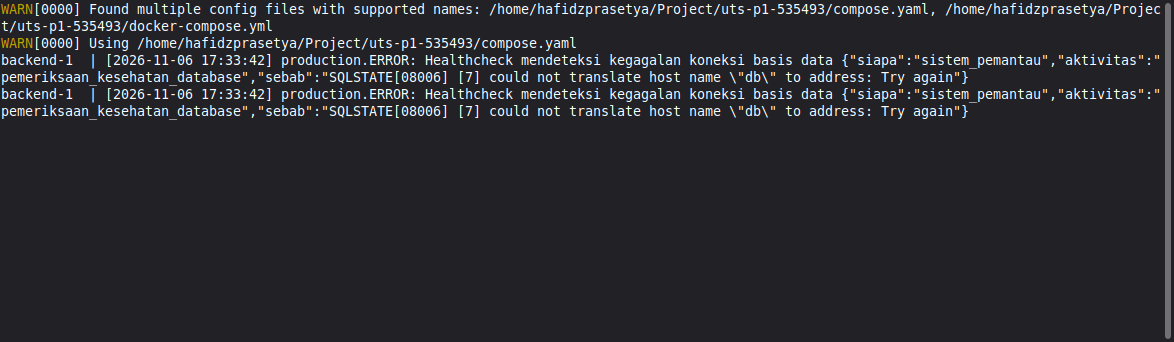
\includegraphics[width=0.98\linewidth,keepaspectratio]{images/ss-02-log-terstruktur.png}}
    \caption{Tangkapan layar potongan ketiga tingkatan log terstruktur pada terminal Linux.}
    \label{fig:log-terstruktur}
\end{figure}

\section{Endpoint Pemeriksaan Kesehatan /health (Soal 3)}
Endpoint \texttt{/health} dirancang untuk memeriksa kesiapan dua komponen vital: koneksi ke basis data PostgreSQL melalui pemanggilan \texttt{DB::connection()->getPdo()} dan pengujian operasi tulis-baca pada subsistem \textit{cache}. Endpoint ini didaftarkan pada berkas \texttt{backend/bootstrap/app.php} secara independen dari middleware sesi web agar tidak terpengaruh oleh dependensi basis data eksternal.

\subsection{Respons Kondisi Sehat (HTTP 200 OK)}
Saat seluruh layanan pendukung beroperasi normal, endpoint \texttt{/health} mengembalikan kode status HTTP 200 OK beserta payload JSON yang menyatakan status \textit{healthy} pada masing-masing subsistem. Bukti pengujian menggunakan perintah \texttt{curl -i http://localhost:8001/health} ditampilkan pada Gambar \ref{fig:health-healthy}.

\begin{figure}[htbp]
    \centering
    \customfbox{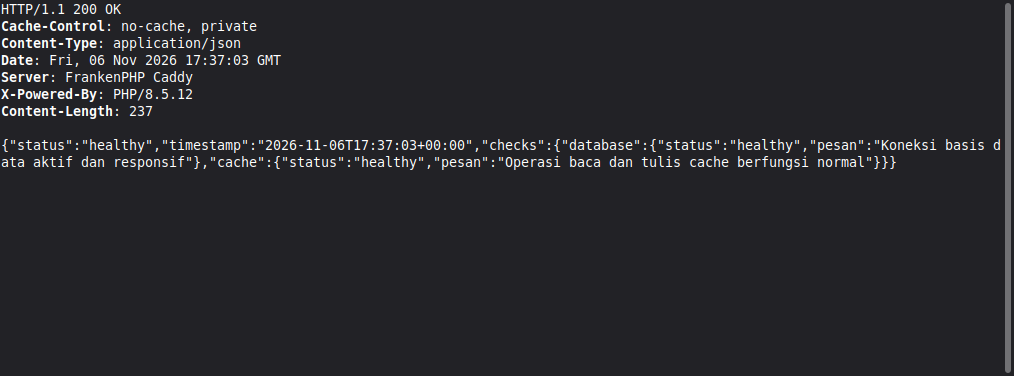
\includegraphics[width=0.98\linewidth,keepaspectratio]{images/ss-03-health-healthy.png}}
    \caption{Isi respons endpoint \texttt{/health} dengan status HTTP 200 OK pada kondisi sehat.}
    \label{fig:health-healthy}
\end{figure}

Struktur balasan JSON yang diterima oleh klien saat kondisi normal adalah sebagai berikut:
\begin{lstlisting}[style=jsonstyle,caption={Payload JSON balasan /health pada kondisi sehat.}]
{
  "status": "healthy",
  "timestamp": "2026-11-06T17:29:02+00:00",
  "checks": {
    "database": {
      "status": "healthy",
      "pesan": "Koneksi basis data aktif dan responsif"
    },
    "cache": {
      "status": "healthy",
      "pesan": "Operasi baca dan tulis cache berfungsi normal"
    }
  }
}
\end{lstlisting}

\subsection{Respons Kondisi Sakit (HTTP 503 Service Unavailable)}
Ketika layanan basis data dimatikan, metode pemeriksaan menangkap kegagalan koneksi PDO, menetapkan status komponen basis data menjadi \textit{unhealthy}, dan menyertakan larik \texttt{bagian\_bermasalah} yang secara tegas menyebutkan subsistem \texttt{database}. Respons yang dikirimkan ke klien memiliki kode status HTTP 503 Service Unavailable, sebagaimana ditunjukkan pada Gambar \ref{fig:health-unhealthy}.

\begin{figure}[htbp]
    \centering
    \customfbox{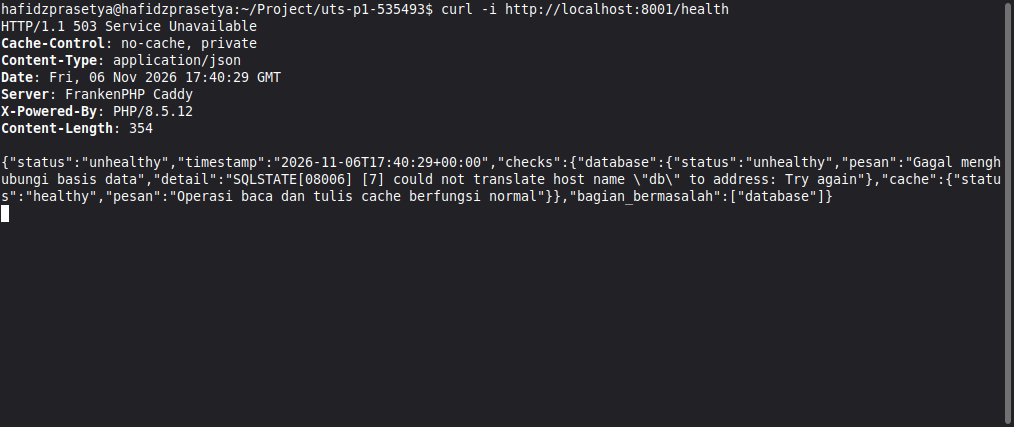
\includegraphics[width=0.98\linewidth,keepaspectratio]{images/ss-05-health-unhealthy.png}}
    \caption{Isi respons endpoint \texttt{/health} dengan status HTTP 503 saat basis data terputus.}
    \label{fig:health-unhealthy}
\end{figure}

Keluaran JSON di bawah menegaskan bahwa subsistem \textit{cache} tetap berstatus sehat, sementara rincian galat koneksi jaringan PostgreSQL dilaporkan secara eksplisit pada bagian \texttt{database}:
\begin{lstlisting}[style=jsonstyle,caption={Payload JSON balasan /health saat basis data mengalami kegagalan.}]
{
  "status": "unhealthy",
  "timestamp": "2026-11-06T17:40:29+00:00",
  "checks": {
    "database": {
      "status": "unhealthy",
      "pesan": "Gagal menghubungi basis data",
      "detail": "SQLSTATE[08006] [7] could not translate host name \"db\" to address: Try again"
    },
    "cache": {
      "status": "healthy",
      "pesan": "Operasi baca dan tulis cache berfungsi normal"
    }
  },
  "bagian_bermasalah": [
    "database"
  ]
}
\end{lstlisting}

\section{Konfigurasi Healthcheck pada Compose (Soal 4)}
Pada berkas orkestrasi \texttt{compose.yaml}, konfigurasi pengujian kesehatan dipasang pada layanan \texttt{backend} dengan memanggil utilitas \texttt{curl} langsung ke endpoint \texttt{/health}. Pengaturan ini dilengkapi dengan parameter \texttt{interval: 10s}, \texttt{timeout: 5s}, \texttt{retries: 5}, dan \texttt{start\_period: 15s}.

\begin{lstlisting}[style=yamlstyle,caption={Konfigurasi healthcheck layanan backend pada compose.yaml.},label={lst:compose-healthcheck}]
backend:
  build: ./backend
  restart: unless-stopped
  environment:
    APP_NAME: "Aset Lab TRPL"
    APP_ENV: production
    APP_DEBUG: "false"
    APP_KEY: ${APP_KEY}
    LOG_CHANNEL: stdout
    CACHE_STORE: file
    SESSION_DRIVER: file
    DB_CONNECTION: pgsql
    DB_HOST: db
    DB_PORT: 5432
    DB_DATABASE: ${DB_DATABASE}
    DB_USERNAME: ${DB_USERNAME}
    DB_PASSWORD: ${DB_PASSWORD}
  depends_on:
    db:
      condition: service_healthy
  ports:
    - "${BACKEND_PORT:-8001}:8000"
  healthcheck:
    test: ["CMD-SHELL", "curl -fs http://localhost:8000/health || exit 1"]
    interval: 10s
    timeout: 5s
    retries: 5
    start_period: 15s
  logging:
    driver: "json-file"
    options:
      max-size: "10m"
      max-file: "3"
\end{lstlisting}

Ketika seluruh kontainer pertama kali dijalankan melalui perintah \texttt{docker compose up -d}, kontainer \texttt{db} dan \texttt{backend} melewati tahap inisialisasi dan berhasil diverifikasi oleh skrip pemeriksa. Keluaran perintah \texttt{docker compose ps} pada Gambar \ref{fig:ps-healthy} membuktikan kolom status kontainer backend dan database bernilai \texttt{Up (healthy)}.

\begin{figure}[htbp]
    \centering
    \customfbox{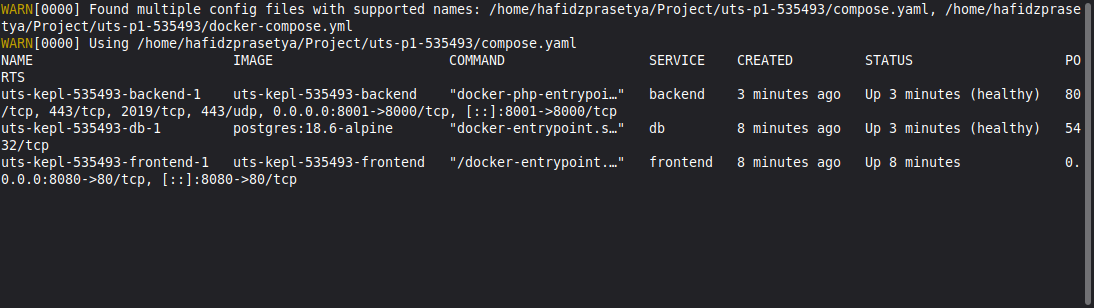
\includegraphics[width=0.98\linewidth,keepaspectratio]{images/ss-04-compose-ps-healthy.png}}
    \caption{Keluaran \texttt{docker compose ps} saat seluruh layanan berstatus \textit{healthy}.}
    \label{fig:ps-healthy}
\end{figure}

\section{Pengujian Pemulihan Dua Arah (Soal 5)}
Untuk membuktikan bahwa mekanisme \textit{healthcheck} bekerja secara dinamis dalam dua arah, layanan basis data sengaja dimatikan menggunakan perintah:
\begin{lstlisting}[style=bashstyle]
docker compose stop db
\end{lstlisting}

Setelah layanan basis data berhenti, pemeriksaan periodik kontainer backend mendeteksi kegagalan koneksi ke host \texttt{db}. Karena endpoint \texttt{/health} merespons dengan kode 503, perintah \texttt{curl -fs} mengembalikan kode galat non-nol (\textit{exit code 1}). Setelah batas percobaan ulang (\texttt{retries: 5}) terlampaui, status kontainer backend pada keluaran \texttt{docker compose ps} otomatis berubah menjadi \texttt{Up (unhealthy)}, sebagaimana terdokumentasi pada Gambar \ref{fig:ps-unhealthy}.

\begin{figure}[htbp]
    \centering
    \customfbox{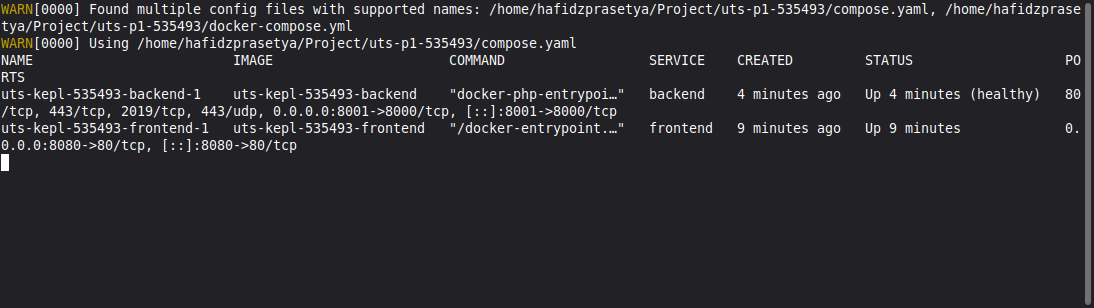
\includegraphics[width=0.98\linewidth,keepaspectratio]{images/ss-06-compose-ps-unhealthy.png}}
    \caption{Keluaran \texttt{docker compose ps} menunjukkan kontainer backend berubah menjadi \textit{unhealthy}.}
    \label{fig:ps-unhealthy}
\end{figure}

Selanjutnya, layanan basis data dihidupkan kembali menggunakan perintah:
\begin{lstlisting}[style=bashstyle]
docker compose start db
\end{lstlisting}

Sesaat setelah kontainer basis data siap menerima koneksi kembali, pemeriksaan \textit{healthcheck} backend berikutnya membuahkan hasil sukses (HTTP 200). Mesin Docker langsung memulihkan status kontainer backend kembali menjadi \texttt{Up (healthy)} tanpa memerlukan tindakan \textit{restart} manual terhadap aplikasi web. Bukti pemulihan otomatis status sehat ini disajikan pada Gambar \ref{fig:ps-recovered}.

\begin{figure}[htbp]
    \centering
    \customfbox{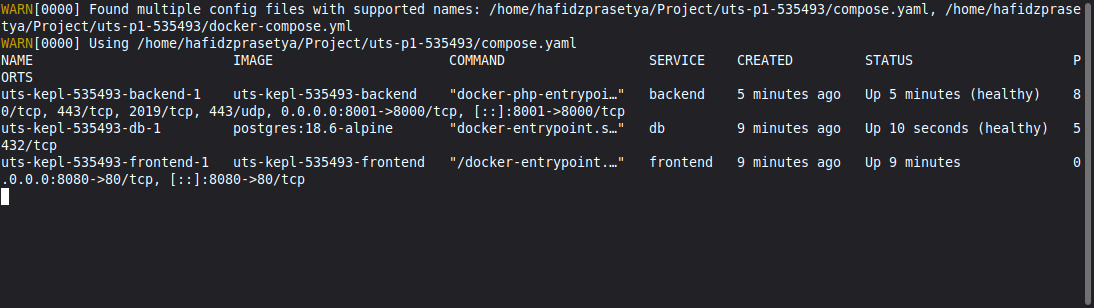
\includegraphics[width=0.98\linewidth,keepaspectratio]{images/ss-07-compose-ps-recovered.png}}
    \caption{Status kontainer backend otomatis kembali \textit{healthy} setelah basis data dihidupkan ulang.}
    \label{fig:ps-recovered}
\end{figure}

\section{Pembatasan Ukuran Berkas Log (Soal 6)}
Pencatatan log aplikasi yang terus-menerus dialirkan ke kontainer berpotensi menghabiskan kapasitas ruang penyimpanan fisik pada server jika tidak dibatasi. Untuk mencegah masalah tersebut, blok konfigurasi \texttt{logging} ditambahkan pada setiap layanan di dalam berkas \texttt{compose.yaml}.

Pengaturan menggunakan driver standar \texttt{json-file} dengan opsi \texttt{max-size: "10m"} yang membatasi ukuran satu berkas log maksimal sebesar 10 Megabyte, serta \texttt{max-file: "3"} yang membatasi retensi rotasi log maksimal sebanyak 3 arsip berkas. Bukti konfigurasi pada berkas deklaratif dan verifikasi inspeksi kontainer melalui perintah \texttt{docker inspect} ditunjukkan pada Gambar \ref{fig:logging-maxsize}.

\begin{figure}[htbp]
    \centering
    \customfbox{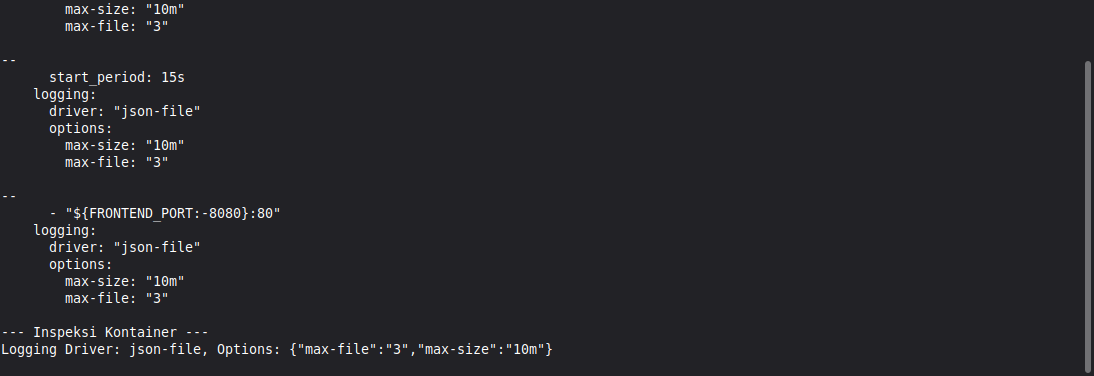
\includegraphics[width=0.98\linewidth,keepaspectratio]{images/ss-08-logging-maxsize.png}}
    \caption{Konfigurasi \texttt{max-size} dan \texttt{max-file} serta hasil inspeksi runtime kontainer.}
    \label{fig:logging-maxsize}
\end{figure}

\section{Penyelarasan Repositori GitHub}
Seluruh penambahan kode pengendali \texttt{HealthController}, pembaruan \texttt{AssetController}, pengujian otomatis \texttt{HealthCheckTest}, serta berkas \texttt{compose.yaml} telah digabungkan ke cabang utama (\texttt{main}) melalui Pull Request nomor 11. Bukti komit terbaru pada repositori publik GitHub ditampilkan pada Gambar \ref{fig:github-commit}.

\begin{figure}[htbp]
    \centering
    \customfbox{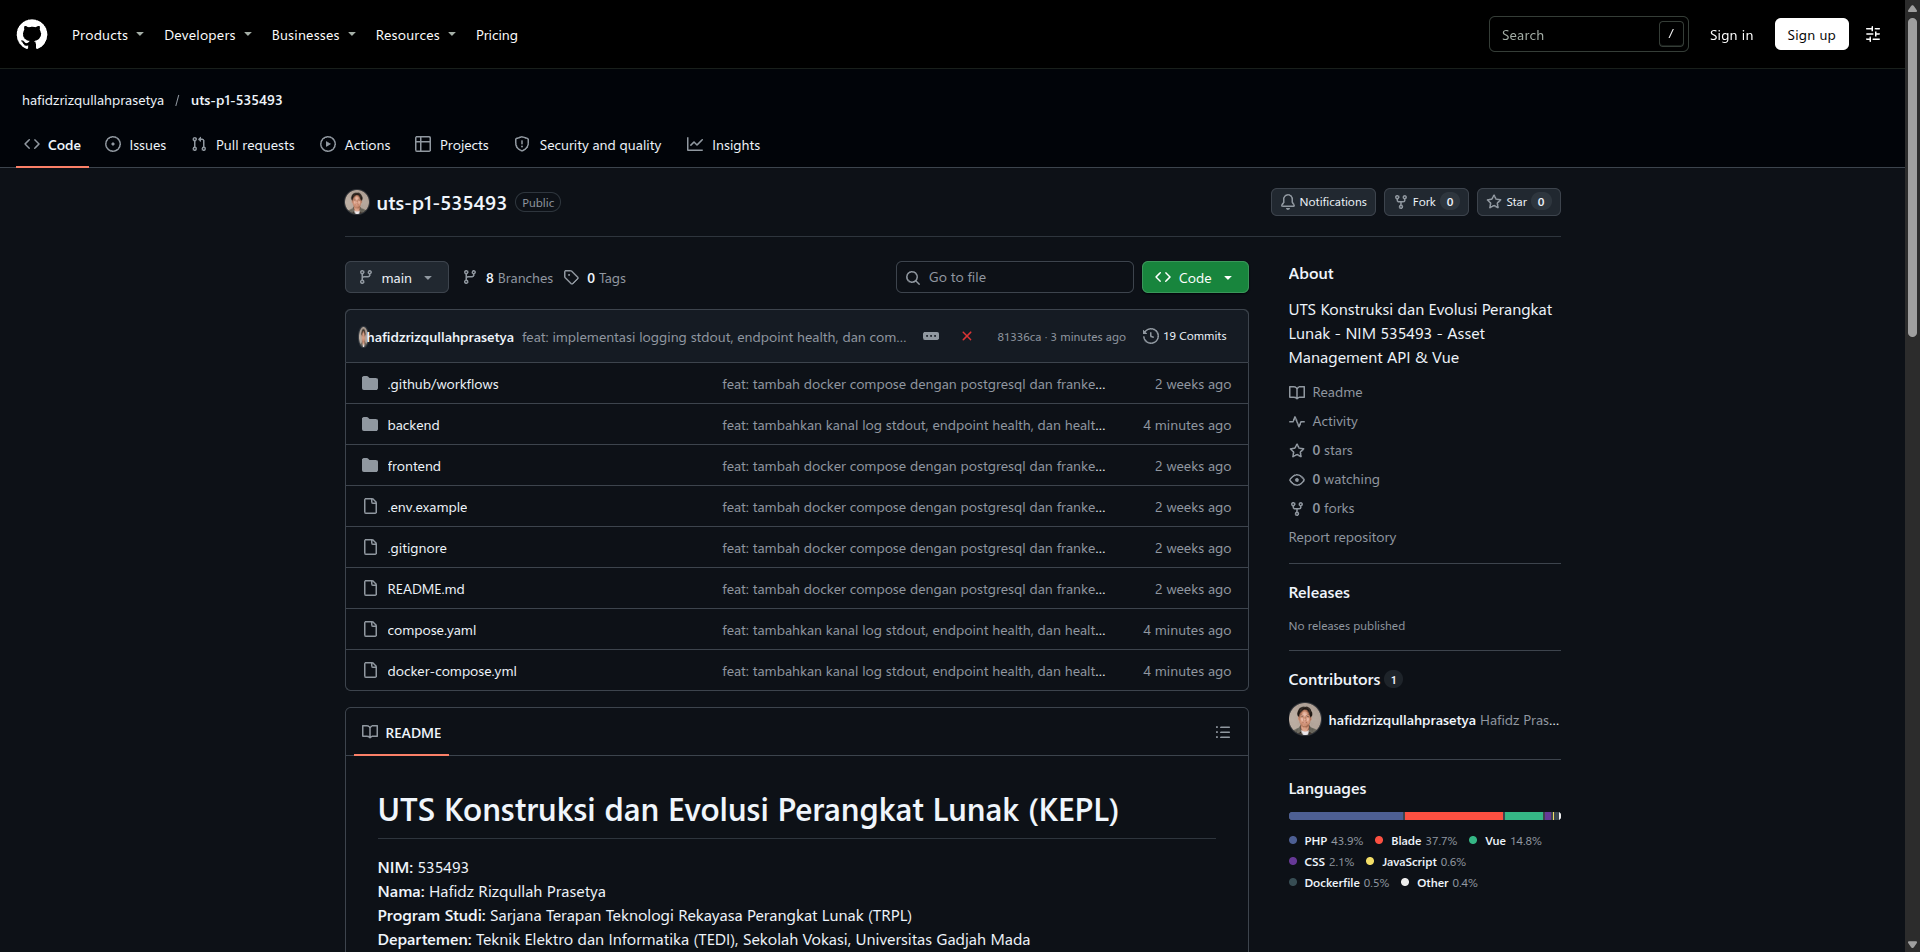
\includegraphics[width=0.98\linewidth,keepaspectratio]{images/ss-09-github-repo-commit.png}}
    \caption{Tampilan repositori publik GitHub memuat pembaruan berkas tugas 6 pada cabang \texttt{main}.}
    \label{fig:github-commit}
\end{figure}

\clearpage

\chapter{Kesimpulan}

Berdasarkan seluruh rangkaian perancangan, implementasi kode, dan pengujian sistem yang telah diselesaikan pada penugasan ini, diperoleh kesimpulan sebagai berikut:
\begin{enumerate}
    \item Konfigurasi kanal pencatatan log pada Laravel berhasil dialihkan ke \texttt{stdout} melalui pengaturan \texttt{StreamHandler} pada berkas \texttt{logging.php} dan variabel lingkungan \texttt{LOG\_CHANNEL=stdout}. Seluruh keluaran log aplikasi berhasil ditangkap langsung oleh perintah \texttt{docker compose logs} tanpa membebani media penyimpanan internal kontainer.
    \item Tiga tingkatan log terstruktur (\texttt{info}, \texttt{warning}, dan \texttt{error}) telah diimplementasikan pada alur penyimpanan data aset, penolakan validasi formulir, dan kegagalan koneksi basis data. Masing-masing entri log membawa konteks pelaku, aktivitas, dan alasan secara terinci dengan tetap menjamin perlindungan privasi tanpa mencatat data kredensial maupun informasi sensitif.
    \item Endpoint \texttt{/health} telah berhasil dibangun dengan memverifikasi kesiapan operasional basis data PostgreSQL dan subsistem penyimpanan \textit{cache}. Endpoint ini secara konsisten mengembalikan kode status HTTP 200 OK saat seluruh komponen sehat, serta mengembalikan kode HTTP 503 Service Unavailable dan merinci komponen yang bermasalah saat terjadi pemutusan koneksi basis data.
    \item Konfigurasi deklaratif \textit{healthcheck} pada \texttt{compose.yaml} dengan interval 10 detik, batas waktu 5 detik, 5 kali percobaan ulang, dan masa tenggang awal 15 detik terbukti andal memantau status operasional kontainer backend. Kolom status pada perintah \texttt{docker compose ps} secara akurat merefleksikan kondisi kesehatan internal aplikasi.
    \item Mekanisme pemantauan kesehatan terbukti bekerja secara adaptif dalam dua arah. Saat layanan basis data dimatikan secara sengaja, kontainer backend bertransisi secara mandiri menjadi berstatus \textit{unhealthy}. Begitu layanan basis data dihidupkan kembali, status kontainer backend otomatis kembali menjadi \textit{healthy} tanpa perlu melakukan intervensi manual terhadap proses peladen web.
    \item Penerapan opsi pembatasan rotasi log dengan driver \texttt{json-file}, \texttt{max-size: "10m"}, dan \texttt{max-file: "3"} berhasil diaktifkan pada lingkungan Docker Compose, menjamin stabilitas konsumsi ruang penyimpanan peladen dari ancaman akumulasi berkas log tak terbatas.
\end{enumerate}

\clearpage

\addcontentsline{toc}{chapter}{Daftar Pustaka}
\begin{thebibliography}{99}
\bibitem{twelve-factor}
A. Wiggins, ``The Twelve-Factor App: XI. Logs - Treat logs as event streams,'' 2017. [Daring]. Tersedia: \url{https://12factor.net/logs}. [Diakses: 06-Nov-2026].

\bibitem{docker-logging}
Docker Inc., ``Configure logging drivers - JSON File logging driver,'' Docker Documentation, 2026. [Daring]. Tersedia: \url{https://docs.docker.com/engine/logging/drivers/json-file/}. [Diakses: 06-Nov-2026].

\bibitem{monolog}
J. Selda, ``Monolog - Logging for PHP 8,'' GitHub Repository, 2026. [Daring]. Tersedia: \url{https://github.com/Seldaek/monolog}. [Diakses: 06-Nov-2026].

\bibitem{owasp-logging}
OWASP Foundation, ``Logging Cheat Sheet - Sensitive Data Protection and Storage,'' OWASP Cheat Sheet Series, 2026. [Daring]. Tersedia: \url{https://cheatsheetseries.owasp.org/cheatsheets/Logging_Cheat_Sheet.html}. [Diakses: 06-Nov-2026].

\bibitem{docker-healthcheck}
Docker Inc., ``Dockerfile reference: HEALTHCHECK instruction,'' Docker Documentation, 2026. [Daring]. Tersedia: \url{https://docs.docker.com/reference/dockerfile/#healthcheck}. [Diakses: 06-Nov-2026].

\bibitem{docker-compose-spec}
Compose Open Source Community, ``Compose file specification: healthcheck attribute,'' 2026. [Daring]. Tersedia: \url{https://docs.docker.com/compose/compose-file/05-services/#healthcheck}. [Diakses: 06-Nov-2026].
\end{thebibliography}

\end{document}
